\section{Intro}\label{sec:intro}

\begin{frame}{What is RxJava?}
	\begin{figure}[h]
		
\includegraphics[width=0.5\textwidth,page=1]{gfx/rx_logo}
	\end{figure}
\end{frame}

\begin{frame}{Types of Concurrency}
	\begin{figure}[h]
		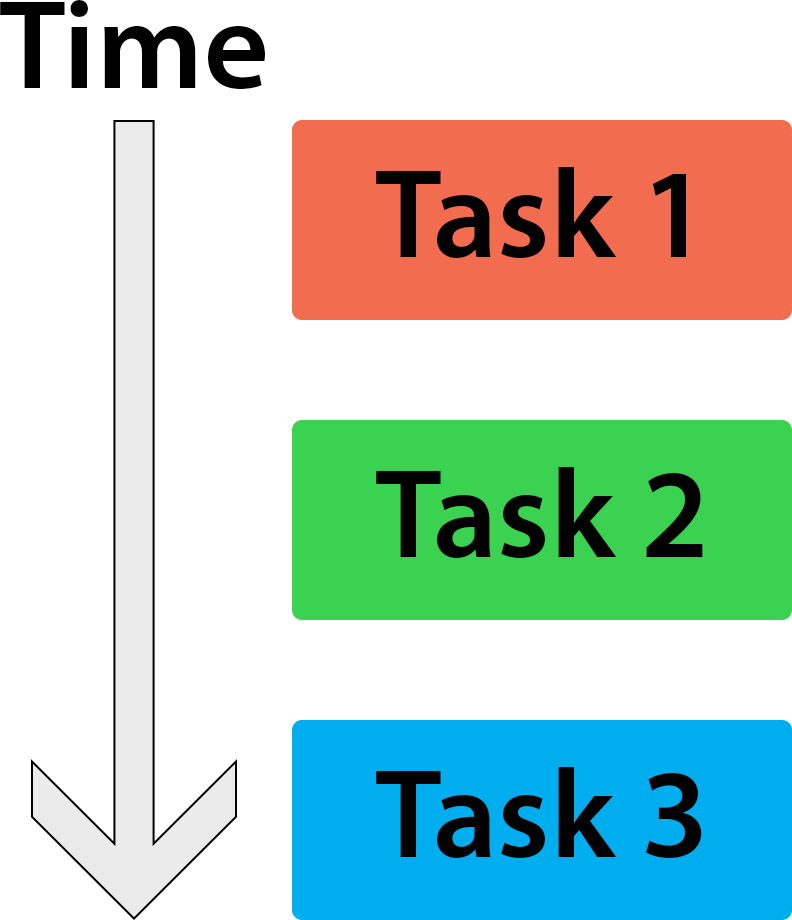
\includegraphics[width=0.6\textwidth,page=1]{gfx/single_threaded_nowait}
	\end{figure}
\end{frame}

\begin{frame}{Types of Concurrency}
	\begin{figure}[h]
		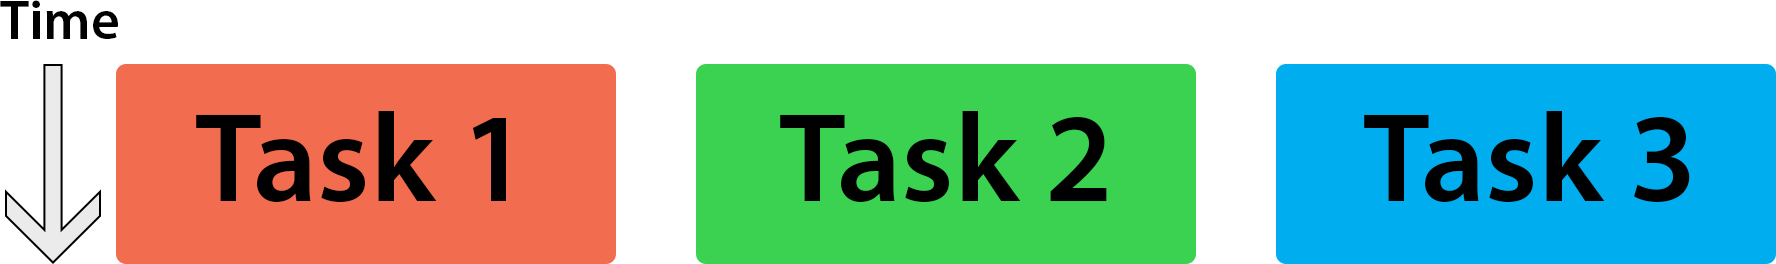
\includegraphics[width=1.0\textwidth,page=1]{gfx/multi_threaded}
	\end{figure}
\end{frame}

\begin{frame}{Types of Concurrency}
	\begin{figure}[h]
		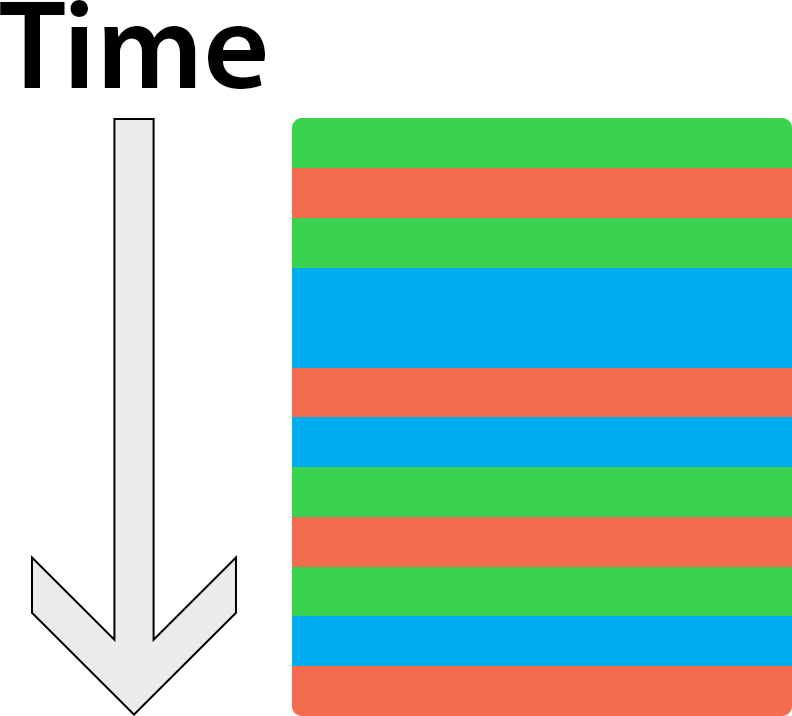
\includegraphics[width=0.7\textwidth,page=1]{gfx/asynchronous_nowait}
	\end{figure}
\end{frame}

\begin{frame}{Types of Concurrency}
	\begin{figure}[h]
		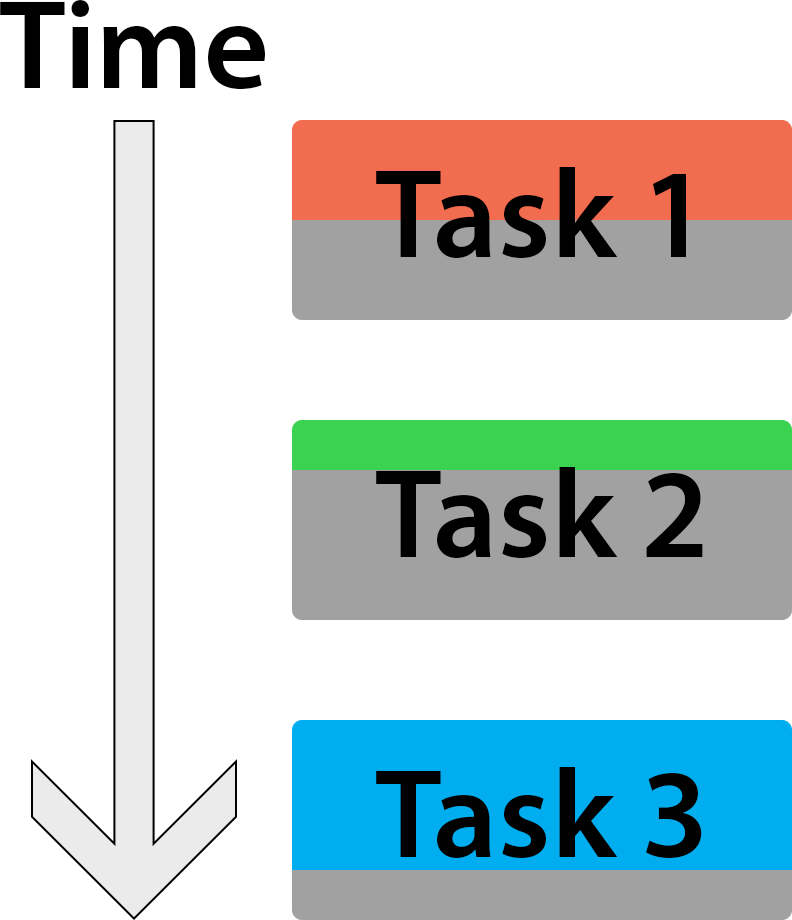
\includegraphics[width=0.6\textwidth,page=1]{gfx/single_threaded_wait}
	\end{figure}
\end{frame}

\begin{frame}[fragile]{Sequential Processing}
    \begin{minted}{python}
                try:
                    for item in collection:
    onNext() ->         doWithAndWaitFor(item)
                except Exception e:
   onError() ->     panic(e)

onComplete() -> cleanup()
    \end{minted}
\end{frame}

\begin{frame}{Types of Concurrency}
	\begin{figure}[h]
		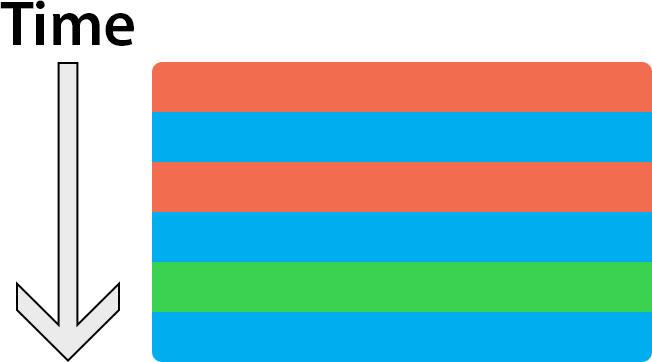
\includegraphics[width=0.7\textwidth,page=1]{gfx/asynchronous_wait}
	\end{figure}
\end{frame}

\begin{frame}{Callback Hell}
	\begin{figure}[h]
		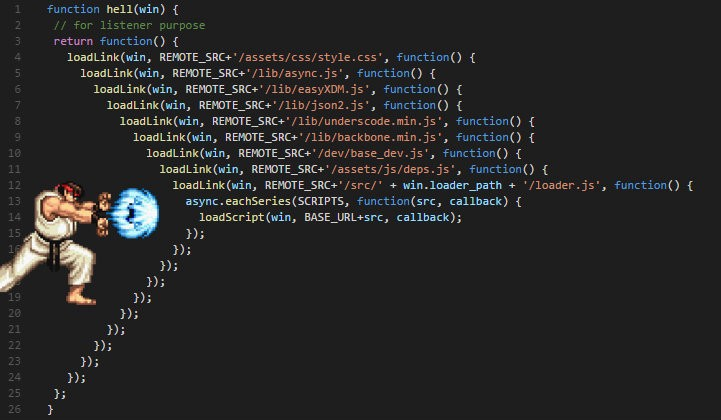
\includegraphics[width=1.0\textwidth,page=1]{gfx/callback_hadouken}
	\end{figure}
\end{frame}

\begin{frame}{Callback Hell - Dante's Inferno}
	\begin{figure}[h]
		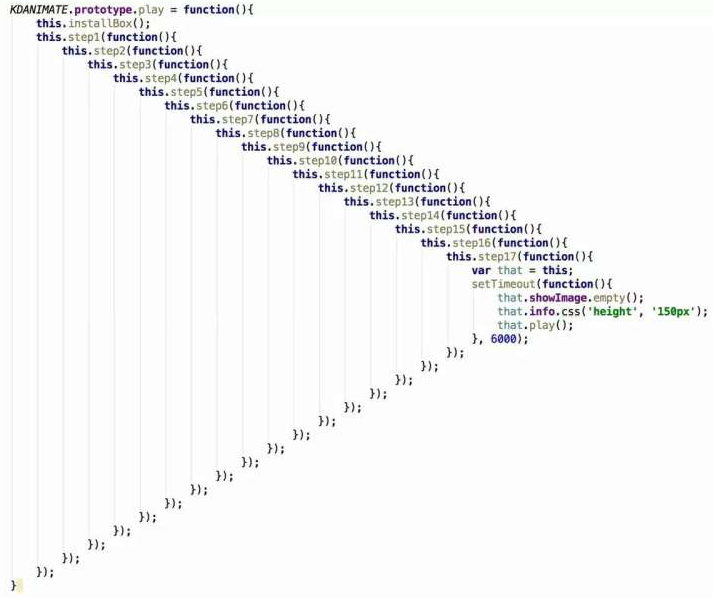
\includegraphics[width=0.9\textwidth,page=1]{gfx/extreme_callback}
	\end{figure}
\end{frame}
